%%%%%%%%%%%%%%%%%%%%%%% file template.tex %%%%%%%%%%%%%%%%%%%%%%%%%
%
% This is a general template file for the LaTeX package SVJour3
% for Springer journals.          Springer Heidelberg 2010/09/16
%
% Copy it to a new file with a new name and use it as the basis
% for your article. Delete % signs as needed.
%
% This template includes a few options for different layouts and
% content for various journals. Please consult a previous issue of
% your journal as needed.
%
%%%%%%%%%%%%%%%%%%%%%%%%%%%%%%%%%%%%%%%%%%%%%%%%%%%%%%%%%%%%%%%%%%%
%
% First comes an example EPS file -- just ignore it and
% proceed on the \documentclass line
% your LaTeX will extract the file if required
\begin{filecontents*}{example.eps}
%!PS-Adobe-3.0 EPSF-3.0
%%BoundingBox: 19 19 221 221
%%CreationDate: Mon Sep 29 1997
%%Creator: programmed by hand (JK)
%%EndComments
gsave
newpath
  20 20 moveto
  20 220 lineto
  220 220 lineto
  220 20 lineto
closepath
2 setlinewidth
gsave
  .4 setgray fill
grestore
stroke
grestore
\end{filecontents*}
%
\RequirePackage{fix-cm}
%
%\documentclass{svjour3}                     % onecolumn (standard format)
\documentclass[smallcondensed]{svjour3}     % onecolumn (ditto)
%\documentclass[smallextended]{svjour3}       % onecolumn (second format)
%\documentclass[twocolumn]{svjour3}          % twocolumn
%
\smartqed  % flush right qed marks, e.g. at end of proof
%
\usepackage{graphicx}
\usepackage{amsmath,amsthm}
%
%\usepackage{mathptmx}      % use Times fonts if available on your TeX system
%
% insert here the call for the packages your document requires
%\usepackage{latexsym}
% etc.
%
% please place your own definitions here and don't use \def but
% \newcommand{}{}
%
% Insert the name of "your journal" with
% \journalname{myjournal}
%
\begin{document}

\title{Approximate Solutions of Initial Value Problems for Ordinary Differential Equations Using Radial Basis Function Networks%\thanks{Grants or other notes
%about the article that should go on the front page should be
%placed here. General acknowledgments should be placed at the end of the article.}
}
%\subtitle{Do you have a subtitle?\\ If so, write it here}

%\titlerunning{Short form of title}        % if too long for running head

\author{Fatma B. Rizaner         \and
        Ahmet Rizaner %etc.
}

%\authorrunning{Short form of author list} % if too long for running head

\institute{F.B. Rizaner \at
              Department of Mathematics, Eastern Mediterranean University, Famagusta, North Cyprus, Mersin 10, Turkey \\
              Tel.: +90-392-3651604\\
              Fax: +90-392-6302281\\
              \email{fatma.bayramoglu@emu.edu.tr}           %  \\
%             \emph{Present address:} of F. Author  %  if needed
           \and
           A. Rizaner \at
              Department of Information Technology, Eastern Mediterranean University, Famagusta, North Cyprus, Mersin 10, Turkey
}

\date{Received: date / Accepted: date}
% The correct dates will be entered by the editor


\maketitle

\begin{abstract}
We present a numerical approach to approximate first order initial value problems (IVP) by using unsupervised radial basis function (RBF) networks. The presented unsupervised model successfully approximates the solutions of IVPs with a high accuracy. The results of the proposed approach are also compared with the results of a previously proposed neural network approximation for representative examples.
\keywords{initial value problems\and ordinary differential equations\and radial basis function network\and artificial neural networks\and function approximation}
% \PACS{PACS code1 \and PACS code2 \and more}
% \subclass{65Y10\and 35E15\and  62M45}
\end{abstract}

\section{Introduction}
\label{intro}
Many problems in science and engineering can be represented in terms of ordinary differential equations (ODEs). Since it is not easy to obtain the exact solutions of ODEs, numerical approaches have been developed. Techniques involving the architectures of artificial neural networks have also great interest in finding the solution of initial value problems (IVPs) \cite{Mal1}\cite{Mal2}\cite{Shir3}\cite{Park4}. A regression based artificial neural network model has been considered in \cite{Mal1} for the solutions of ODEs. It has been shown by examples that the approximate results of the neural model are very accurate \cite{Mal1}. In \cite{Mal2}, a new neural network based solution of IVPs by the use of Legendre polynomials has been developed. Another scheme based on the unsupervised version of kernel least mean square algorithm has been implemented by Yazid et al. for the solution of ODEs \cite{Shir3}. It has been reported that radial basis function (RBF) networks are capable of universal approximation even with a single hidden layer \cite{Park4}. A fuzzy wavelet neural network based approximation approach of the first order partial derivatives is also considered in \cite{Nejad6}. The generalization ability of multi-layer back propagation and reformulated RBF network has been compared by Choi and Lee \cite{Choi5}. It has been concluded that reformulated RBF networks with a supervised learning have better performance in convergence and generalization for solving differential equations \cite{Choi5}.

In this paper, we propose a new approach based on RBF networks for solving ODEs. The approximate solution, whose parameters are adjusted to minimize an appropriate error function, is presented in the closed form by means of RBFs. Some numerical examples are also presented to illustrate the efficiency of the proposed method.

The rest of the paper is organized as follows. Section 2 presents the proposed RBF network model. In Section 3, we discuss the application of RBF network to solve first order IVPs. Section 4 presents numerical results and their discussions. Finally, in Section 5 we conclude with a final overview of the obtained results.

% Figure 1 
\begin{figure}
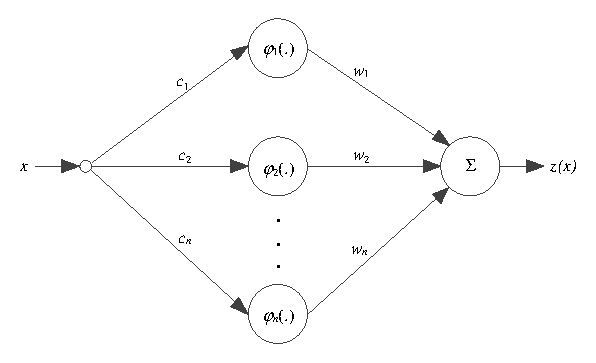
\includegraphics[width=9.5cm]{Fig1.eps}
\caption{Architecture of a radial basis function network}
\label{fig1}      
\end{figure}

% Table 1
\begin{table}[h]
\caption{Exact solution and approximation of proposed unsupervised RBF based network for example 1}
\label{Table1}
\begin{tabular}{llllll}
$t$ & $y(t)$ & \begin{tabular}[c]{@{}l@{}}RBF Net.\\ ($n=3$)\end{tabular} & \begin{tabular}[c]{@{}l@{}}RBF Net.\\ ($n=5$)\end{tabular} & \begin{tabular}[c]{@{}l@{}}RBF Net.\\ ($n=7$)\end{tabular} & \begin{tabular}[c]{@{}l@{}}RBF Net.\\ ($n=9$)\end{tabular} \\
\hline\noalign{\smallskip}
0.00 & 1.0000 & 1.0000 & 1.0000 & 1.0000 & 1.0000 \\
0.05 & 0.9536 & 0.9500 & 0.9543 & 0.9536 & 0.9536 \\
0.10 & 0.9137 & 0.9111 & 0.9144 & 0.9137 & 0.9137 \\
0.15 & 0.8798 & 0.8800 & 0.8799 & 0.8798 & 0.8798 \\
0.20 & 0.8514 & 0.8547 & 0.8507 & 0.8514 & 0.8514 \\
0.25 & 0.8283 & 0.8344 & 0.8269 & 0.8283 & 0.8283 \\
0.30 & 0.8104 & 0.8184 & 0.8086 & 0.8104 & 0.8104 \\
0.35 & 0.7978 & 0.8067 & 0.7958 & 0.7978 & 0.7978 \\
0.40 & 0.7905 & 0.7995 & 0.7887 & 0.7905 & 0.7905 \\
0.45 & 0.7889 & 0.7971 & 0.7874 & 0.7889 & 0.7889 \\
0.50 & 0.7931 & 0.7999 & 0.7921 & 0.7931 & 0.7930 \\
0.55 & 0.8033 & 0.8081 & 0.8028 & 0.8034 & 0.8033 \\
0.60 & 0.8200 & 0.8222 & 0.8197 & 0.8200 & 0.8199 \\
0.65 & 0.8431 & 0.8426 & 0.8429 & 0.8432 & 0.8431 \\
0.70 & 0.8731 & 0.8697 & 0.8726 & 0.8732 & 0.8731 \\
0.75 & 0.9101 & 0.9040 & 0.9088 & 0.9101 & 0.9100 \\
0.80 & 0.9541 & 0.9460 & 0.9519 & 0.9541 & 0.9540 \\
0.85 & 1.0053 & 0.9962 & 1.0021 & 1.0053 & 1.0052 \\
0.90 & 1.0637 & 1.0552 & 1.0598 & 1.0637 & 1.0637 \\
0.95 & 1.1293 & 1.1237 & 1.1254 & 1.1294 & 1.1293 \\
1.00 & 1.2022 & 1.2022 & 1.1991 & 1.2022 & 1.2021 \\
\hline\noalign{\smallskip}
\multicolumn{2}{l}{Average MSE :} & $3.48\times10^{-05}$ & $3.54\times10^{-06}$ & $7.75\times10^{-10}$ & $6.80\times10^{-10}$
\end{tabular}
\end{table}

\section{Radial Basis Function (RBF) Network Model}
\label{sec:2}

The architecture of the considered radial basis function network model with three layers is shown in Figure~\ref{fig1}. The first layer of network performs a non-linear transformation of the input with the non-linear Gaussian basis activation functions \cite{Chen6}. The {\it{i}}-th RBF can be represented as:

% Equation 1
\begin{equation}
{\varphi_{i}=e^{-\frac{(x-c_{i})^{2}}{\sigma^{2}}}},
\end{equation}

\noindent
where $x$ is the input of the network, $c_i$ and $\sigma$ represents the {\it{i}}-th center and width of the Gaussians basis functions respectively. The output of the RBF network is the linear combination of the outputs from $n$ radial basis functions weighted by appropriate coefficients (${w_j}$),

% Equation 2
\begin{equation}
{z(x)=\sum_{J=1}^{n}w_j\varphi_j(x)}.
\end{equation}


\section{Unsupervised RBF network solution of first order IVPs}
\label{sec:3}

A first-order initial value problem could be formulated as:

% Equation 3
\begin{equation}
\frac{\partial y(x)}{\partial x}=f(x,y), x\in [a,b]
\end{equation}

\noindent
with the initial condition $y(a)=A$.

We can define a trial solution for (3) as sum of two terms in the following form:

% Equation 4
\begin{equation}
y_T (x)=A+(x-a)z(x).
\end{equation}

The error function of the approximation can be defined as the square of the error between the derivative of the trial and exact solution as:

% Equation 5
\begin{equation}
E(w)=\frac{1}{2}\left [ \frac{\partial y_T(x))}{\partial x}-f(x,y) \right ]^{2}.
\end{equation}

The weight coefficients of the RBF network is updated starting with initial random weight to minimize (5) with the gradient descent method as:

% Equation 6
\begin{equation}
w_j^k=w_j^{k-1}-\eta \frac{\partial E(w)}{\partial w_j^k},
\end{equation}

\noindent
where $\eta$ is the learning rate parameter, $k$ is the iteration index and, \\${\partial E(w)}/{\partial w_j^k}$ can be calculated as:

% Equation 7
\begin{equation}
\begin{split}
\frac{\partial E(w)}{\partial w_j^k}=\left ( 1-\frac{2}{\sigma ^{2}}(x-c_j)^{2}(x-a)e^{-\frac{(x-c_{j})^{2}}{\sigma^{2}}} \right)\times \\
\left ( \sum_{i=1}^{n}( 1-\frac{2}{\sigma ^{2}}(x-c_i)^{2}(x-a)w_i^ke^{-\frac{(x-c_{i})^{2}}{\sigma^{2}}})-f(x,y) \right ).
\end{split}
\end{equation}


The proposed algorithm is unsupervised because target solution is not known and generated by iterating the algorithm to minimize $E(w)$.


% Table 2
\begin{table}[h]
\caption{Comparison of exact solution and approximation approaches for example 1}
\label{Table2}
\scalebox{0.90}{
\begin{tabular}{lllllll}
$t$ & $y(t)$ & Euler & Runge-Kutta & MLP-A & MLP-R & \begin{tabular}[c]{@{}l@{}}RBF Net.\\ ($n=9$)\end{tabular} \\
\hline\noalign{\smallskip}
0.00 & 1.0000 & 1.0000 & 1.0000 & 1.0000 & 1.0000 & 1.0000 \\
0.05 & 0.9536 & 0.9500 & 0.9536 & 0.9886 & 0.9677 & 0.9536 \\
0.10 & 0.9137 & 0.9072 & 0.9138 & 0.9084 & 0.9159 & 0.9137 \\
0.15 & 0.8798 & 0.8707 & 0.8799 & 0.8906 & 0.8815 & 0.8798 \\
0.20 & 0.8514 & 0.8401 & 0.8515 & 0.8587 & 0.8531 & 0.8514 \\
0.25 & 0.8283 & 0.8150 & 0.8283 & 0.8309 & 0.8264 & 0.8283 \\
0.30 & 0.8104 & 0.7953 & 0.8105 & 0.8013 & 0.8114 & 0.8104 \\
0.35 & 0.7978 & 0.7810 & 0.7979 & 0.7999 & 0.7953 & 0.7978 \\
0.40 & 0.7905 & 0.7721 & 0.7907 & 0.7918 & 0.7894 & 0.7905 \\
0.45 & 0.7889 & 0.7689 & 0.7890 & 0.7828 & 0.7845 & 0.7889 \\
0.50 & 0.7931 & 0.7717 & 0.7932 & 0.8047 & 0.7957 & 0.7930 \\
0.55 & 0.8033 & 0.7805 & 0.8035 & 0.8076 & 0.8041 & 0.8033 \\
0.60 & 0.8200 & 0.7958 & 0.8201 & 0.8152 & 0.8204 & 0.8199 \\
0.65 & 0.8431 & 0.8178 & 0.8433 & 0.8319 & 0.8399 & 0.8431 \\
0.70 & 0.8731 & 0.8467 & 0.8733 & 0.8592 & 0.8711 & 0.8731 \\
0.75 & 0.9101 & 0.8826 & 0.9102 & 0.9129 & 0.9151 & 0.9100 \\
0.80 & 0.9541 & 0.9258 & 0.9542 & 0.9755 & 0.9555 & 0.9540 \\
0.85 & 1.0053 & 0.9763 & 1.0054 & 1.0056 & 0.9948 & 1.0052 \\
0.90 & 1.0637 & 1.0342 & 1.0638 & 1.0714 & 1.0662 & 1.0637 \\
0.95 & 1.1293 & 1.0995 & 1.1294 & 1.1281 & 1.1306 & 1.1293 \\
1.00 & 1.2022 & 1.1721 & 1.2022 & 1.2108 & 1.2058 & 1.2021 \\
\hline\noalign{\smallskip}
\multicolumn{2}{l}{Average MSE:} & $4.60\times10^{-04}$ & $1.24\times10^{-08}$ & $1.26\times10^{-04}$ & $2.01\times10^{-05}$ & $6.80\times10^{-10}$
\end{tabular}
}
\end{table}


% Figure 2
\begin{figure}
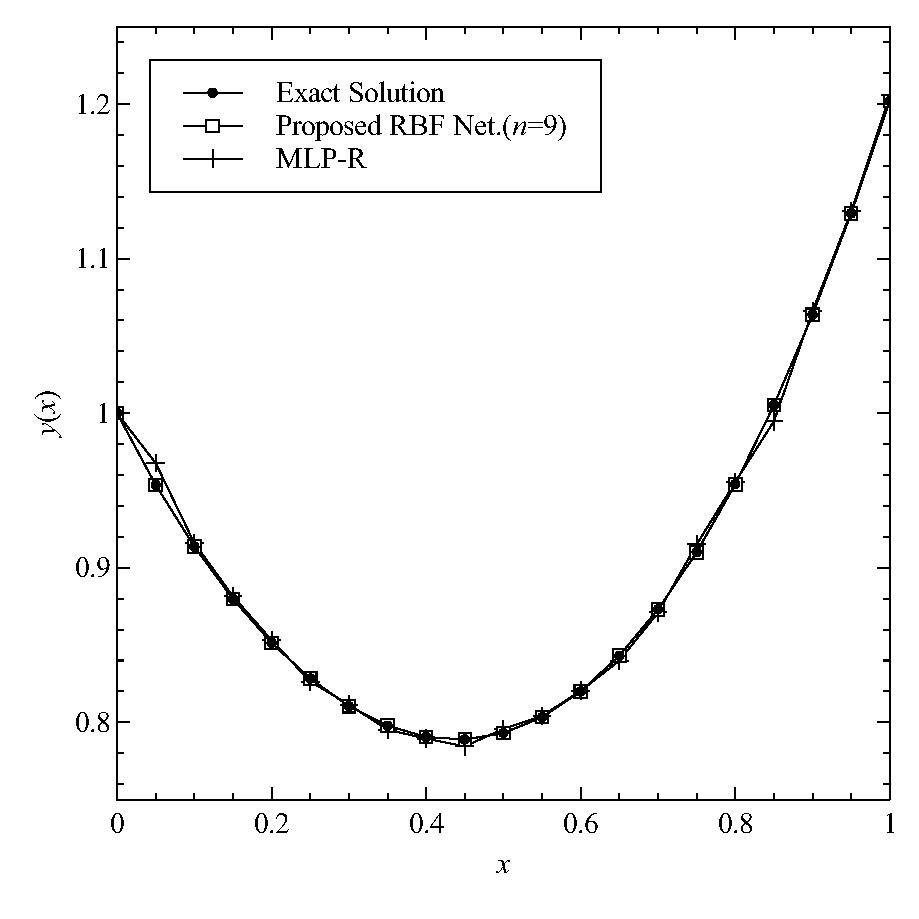
\includegraphics[width=9.5cm]{Fig2.eps}
\caption{Exact solution and approximations of example 1}
\label{fig2}
\end{figure}


\section{Numerical Examples}
\label{sec:4}

In this section, we consider two examples to illustrate the performance of the proposed RBF based unsupervised approximation approach. The estimation accuracies of the presented approaches are calculated by means of average mean squared error (MSE) as,

% Equation 8
\begin{equation}
E_{mse}=\frac{1}{n_s}\sum_{j=1}^{ns}\left ( y(x_j)-y_T(x_j) \right )^{2},
\end{equation}

\noindent
where $n_s$ is the total number of test points and $x_j$ represents the {\it{j}}-th test input.

\subsection{Example 1}

Consider the following first order ODE with time varying coefficient as follow:

% Equation 9
\begin{equation}
\frac{\partial y(x)}{\partial x} + \left ( x + \frac{1+ 3x^2}{1+x+x^3}  \right )y(x)=2x+x^3+x^2\left (  \frac{1+ 3x^2}{1+x+x^3}  \right ), x\in [0 , 1]
\end{equation}

\noindent
with initial condition $y(0)=1$.

The approximate solutions obtained by the proposed approach are compared with the exact solution in Table 1. The approximate solutions are obtained with the different number of RBFs (3, 5, 7 and 9) having constant widths of 0.8 and the centers of the first layer are uniformly distributed inside [0, 1]. A variable learning rate factor is employed for the second layer which decreases linearly with increasing iteration number from 0.2 to 0005. It is clearly seen from Table 1 that increasing number of RBFs improves the estimation performance. The average MSE is obtained as $6.8\times10^{-10}$ with 9 RBFs. Increasing the number of RBFs beyond 9 does not improve the performance significantly.

The results obtained with 9 RBFs are also compared with the results obtained by multi-layer perceptron (MLP) based neural methods of \cite{Mal1} with arbitrary weights (MLP-A) and regression-based weights (MLP-R). Table 2 compares the exact solution with the approximation of the proposed method, MLP based approach, and also with the well-known Euler and Runge-Kutta numerical methods. As clearly seen from the results presented in Table 2, proposed RBF based network outperforms all the other approaches.

The approximate solution obtained with the proposed method is also compared with the exact solution and the approximation of MLP-R in Figure~\ref{fig2}. There is a perfect agreement with the exact solution and the approximate solution obtained by the proposed approach.


%Table 3
\begin{table}[h]
\caption{Exact solution and approximation of proposed unsupervised RBF based network for example 2}
\label{Table3}
\begin{tabular}{lllll}
$t$ & $y(t)$ & \begin{tabular}[c]{@{}l@{}}RBF Net.\\ ($n=9$)\end{tabular} & \begin{tabular}[c]{@{}l@{}}RBF Net.\\ ($n=15$)\end{tabular} & \begin{tabular}[c]{@{}l@{}}RBF Net.\\ ($n=21$)\end{tabular} \\
\hline\noalign{\smallskip}
0.00 & 3.0000 & 3.0000 & 3.0000 & 3.0000 \\
0.15 & 2.3438 & 2.3056 & 2.3447 & 2.3435 \\
0.30 & 1.8142 & 1.4605 & 1.8155 & 1.8138 \\
0.45 & 1.3511 & 0.8294 & 1.3490 & 1.3510 \\
0.60 & 0.9348 & 0.5047 & 0.9312 & 0.9344 \\
0.75 & 0.5763 & 0.4158 & 0.5743 & 0.5752 \\
0.90 & 0.3012 & 0.4280 & 0.3015 & 0.2998 \\
1.05 & 0.1318 & 0.4214 & 0.1324 & 0.1308 \\
1.20 & 0.0726 & 0.3380 & 0.0710 & 0.0720 \\
1.35 & 0.1038 & 0.1914 & 0.0985 & 0.1030 \\
1.50 & 0.1845 & 0.0420 & 0.1757 & 0.1834 \\
1.65 & 0.2643 & -0.0441 & 0.2539 & 0.2632 \\
1.80 & 0.2988 & -0.0343 & 0.2900 & 0.2982 \\
1.95 & 0.2638 & 0.0510 & 0.2589 & 0.2637 \\
2.10 & 0.1625 & 0.1469 & 0.1614 & 0.1622 \\
2.25 & 0.0235 & 0.1737 & 0.0237 & 0.0227 \\
2.40 & -0.1095 & 0.0771 & -0.1109 & -0.1107 \\
2.55 & -0.1937 & -0.1374 & -0.1966 & -0.1952 \\
2.70 & -0.2025 & -0.3881 & -0.2032 & -0.2043 \\
2.85 & -0.1348 & -0.5207 & -0.1300 & -0.1373 \\
3.00 & -0.0157 & -0.3263 & -0.0099 & -0.0186 \\
\hline\noalign{\smallskip}
\multicolumn{2}{l}{Average MSE:} & $6.67\times10^{-2}$ & $1.96\times10^{-5}$ & $1.44\times10^{-6}$
\end{tabular}

\end{table}

% Figure 3
\begin{figure}
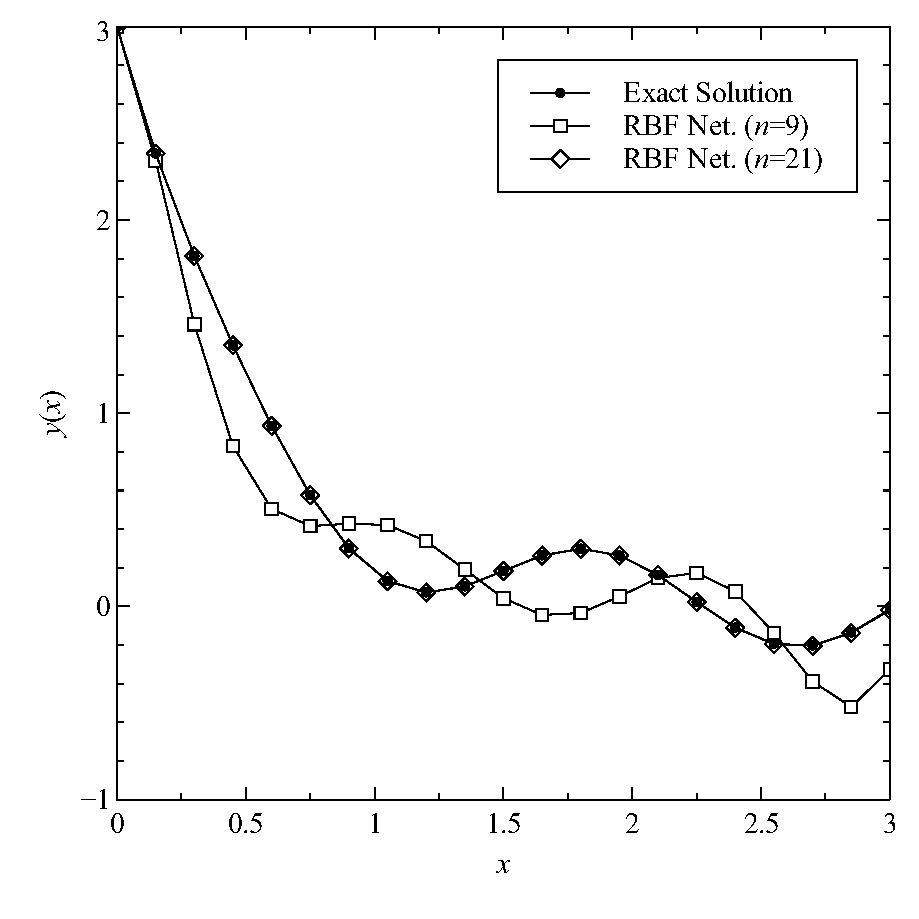
\includegraphics[width=9.5cm]{Fig3.eps}
\caption{Exact solution and approximations of the proposed approach for example 2.}
\label{fig3}
\end{figure}

\subsection{Example 2}

Consider the following first order ODE with time varying coefficient as follow:

% Equation 10
\begin{equation}
\frac{\partial y(x)}{\partial x}+2y(x)=cos(4x), x \in [0 , 3]
\end{equation}

\noindent
with initial condition $y(0)=3$.

Table 3 compares the approximate solutions obtained by the proposed approach with 9, 15 and 21 RBFs with the exact solution. The centers of the first layer are uniformly distributed inside [0, 3], other network parameters are used as explained in example 1. The approximation obtained by 9 RBFs is not acceptable. Increasing the number of RBFs to 15 improves the average MSE of the approximations from $6.67\times10^{-2}$ to $1.96\times10^{-5}$. A better approximation is obtained by increasing the number of RBFs to 21 with an average MSE of $6.8\times10^{-10}$. Increasing the number of RBFs beyond 21 improves the performance slightly. Figure~\ref{fig3} is a different way of comparing the approximations. As seen from this figure, the approximate result obtained with 21 RBFs is very close to the exact solution, however, the approximation obtained with 9 RBFs is not promising.


\section{Conclusion}

In this paper, an unsupervised RBF network model has been developed for solving ordinary differential equations with initial values. The accuracy of the RBF network based approach has been examined by representative examples and compared with some previously proposed neural network based approaches. It has been shown that the proposed approximation method can estimate the solutions of the first order IVPs successfully with a very high accuracy.



%\begin{acknowledgements}
%If you'd like to thank anyone, place your comments here
%and remove the percent signs.
%\end{acknowledgements}

% BibTeX users please use one of
%\bibliographystyle{spbasic}      % basic style, author-year citations
\bibliographystyle{spmpsci}      % mathematics and physical sciences
%\bibliographystyle{spphys}       % APS-like style for physics
%\bibliographystyle{acm}          % acm
\bibliography{mybibfile}          % name your BibTeX data base

% Non-BibTeX users please use
%\begin{thebibliography}{}
%
% and use \bibitem to create references. Consult the Instructions
% for authors for reference list style.
%
%\bibitem{RefJ}
% Format for Journal Reference
%Author, Article title, Journal, Volume, page numbers (year)
% Format for books
%\bibitem{RefB}
%Author, Book title, page numbers. Publisher, place (year)
% etc
%\end{thebibliography}

\end{document}
% end of file template.tex

